\documentclass{article}
\usepackage[utf8]{inputenc}

\title{PS6}
\author{Audrey Hopewell }
\date{3/3/2020}

\usepackage{graphicx}
\usepackage{hyperref}

\begin{document}

\maketitle

\section{Data Cleaning}
I used three \href{https://datasets.imdbws.com/}{datasets} from IMDB. The first had information about type of media, primary/original title, whether the media was "adult," release year, genre, and run time. I filtered the data to only include movies because this is what I'm interested in. I also filtered out titles with release dates of 2020 or later, since only the titles for those movies are available. The second dataset from IMDB had information about average rating and number of ratings on the site. I eliminated movies with fewer than 1000 ratings because average ratings are less meaningful for less-reviewed movies. Then, I merged the two data sets to see if there was any relationship between rating and run-time.

\section{Visualizations}


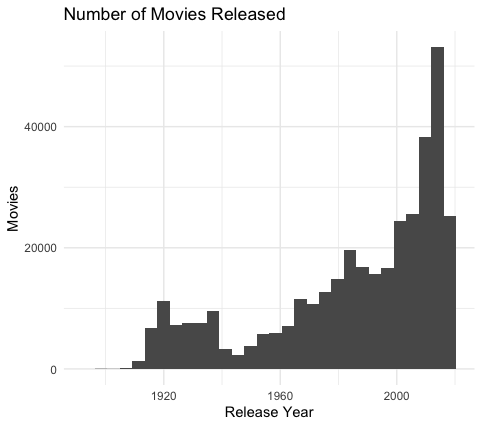
\includegraphics[scale=.7]{PS6a_Hopewell.png}

\caption{This graph shows trends in how many movies are released each year. We can see that there was a dip during the Great Depression and a steady increase (for the most part) since.}

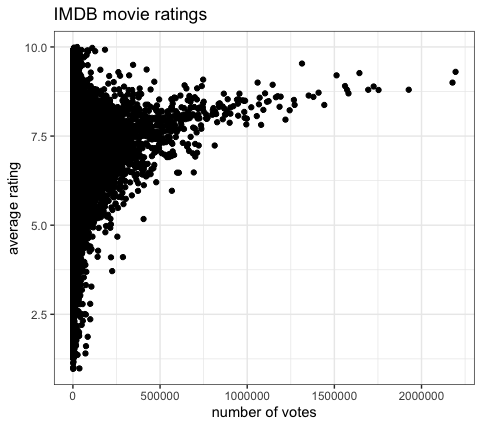
\includegraphics[scale = .7]{PS6b_Hopewell.png}

\caption{This graph shows that movies with more ratings on IMDB tend to have very high average ratings. Most movies with extremely low averages have few ratings.}

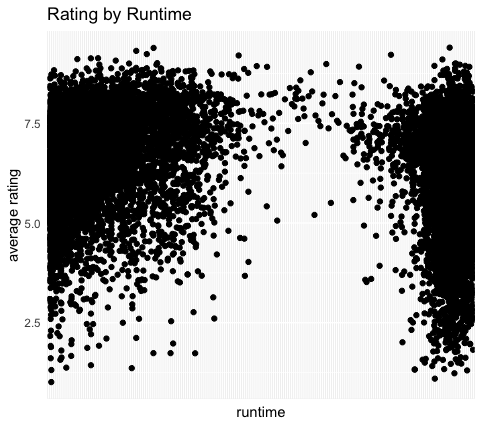
\includegraphics[scale=.7]{PS6c_Hopewell.png}

\caption{This graph shows that very short and very long movies have a lot of variation in their average rating, while those in the middle are consistently fairly high.}

\end{document}
